%
%
%
\chapter{The damped propagator of spin density waves}
\label{ch: propagator}
%
%
%
In the present chapter the propagator of spin density waves should be computed up to the first order in pertubation theory.
The main goal of this masterthesis is the determination of the conductivity for the spin fermion model pertubated via umklapp scattering.
These processes are determined by spin density waves, see section \dots \todo{link to umklapp scattering}, why the propagator of them is needed in the calculation of the conductivity.

Firstly the free spin density wave propagtor is computed.
Therefore the equation of motion of Green functions is used. 
An good introduction of this method can be find in every textbook about quantum field theory in many body physics, but the book by Elk and Gasser \cite{Elk&Gasser} is recommended.
Afterwards the damped propagator is calculated using pertubation theory up the first order.
Finally the obtained propagator is transformed into the Matsubara frequency space.
An easy way to do this is using the Kramer-Kronig relations \eqref{eq: Kramer-Kronig relation}.
%
%
\section{The free propagator of spin density waves}
\label{sec: free propagator}
%
%
In \ref{sec: linear response theory} the linear response theory is established and the retarded susceptibility is introduced this way.
A susceptibility describes the dynamical behaviour of an operator dependent on an external pertubation.
This quantity is close related with the Green function of particles which is called propagator.
The only difference is that the operators and the expectation value of the Green function are represented in the Heisenberg picture comparing to the susceptibility, where they are represented with respect to the unpertubated system.

The Green function's equation of motion is easy to get.
Therefore the Green function has only to be derivated with respect to the time.
The amazing result is that the equation of motion is equally for all typs (retarded, advanced and causal) of Green functions.
Only the boundary conditions are different.
The obtained equation of motion and the boundary conditions are transformed in Fourier space.
%
\begin{align}
	\omega \green{\mt{A}}{\mt{B}}_{\omega}^{j} = \expval*{\comm{\mt{A}}{\mt{B}}_{\eta}} + \green{\comm{\mt{A}}{\mt{H}}_{-}}{\mt{B}}_{\omega}^{j}
	\label{eq: algebraic equation chain}
\end{align}
%
where $j$ labels the typ of the Green function (retarded, advanced and causal) and $\omega$ represented that the Green function is in frequency space.
The double angle brackets symbolized the Green function of the operators A and B.
This equation is an algebraic equation or more precisely an infinite algebraic equation chain for the green function.
On the right hand side in general a new more complicated Green function appears.
For this one exists a new equation chain with a more complicted Green function on the right hand side and so on.
In the case of free propagators we are mostly lucky.
The appearing Green function isn't really complicated, so that the initial Green function appears after one or two interativ steps.
Naturally the same procedure can be done for the Green function in Matsubara time representation.
The result is similar to the one above, only the frequency $\omega$ is replaced with the Matsubara frequancy $i\omega_{n}$.
The simplicity and advantage of this method instead of other ones is that only commutator relations of the (field) operators are needed.
Equation \eqref{eq: algebraic equation chain} is all we need to compute the free propagator of spin density waves.

The dynamic of free spin density waves is described by the Hamiltonian $\mt{H}_{\Phi}$, introduced in chapter \ref{ch: spin fermion model}.
Inserting $\mt{H}_{\Phi}$ and bosonic field operators $\Phi_{\mu}$ for A and B in equation \eqref{eq: algebraic equation chain} is the starting point of the following calculation.
Therefore the abbreviation $\green{\Phi_{\mu}}{\Phi_{\mu}}_{\omega}$ is introduced, where the first operator is readed with the momentum argument $\vb{k}+\vb{G}$ and in comparison the second operator is readed with the opposite one, $-\vb{k}-\vb{G}$.
The time argument is equal in both cases, why it is dropped.
%
\begin{align}
	\omega \green{\Phi_{\mu}}{\Phi_{\mu}}_{\omega} &= 
		\expval{\comm{\Phi_{\mu}(\vb{k}+\vb{G})}{\Phi_{\mu}(-\vb{k}-\vb{G})}}
		+
		\green{\comm{\Phi_{\mu}(\vb{k}+\vb{G})}{\mt{H}_{\Phi}}}{\Phi_{\mu}}_{\omega}
		\label{eq: equation chain SDW}
\end{align}
%

The bosonic commutator relations are given in equation (\dots\todo{link zu bosonischen Vertauschungsrelationen}).
The only non-vanishing commutator relation is that between the bosonic field operator and the corresponding canonical momentum operator.
Therefore on the right hand side of \eqref{eq: equation chain SDW} the inhomogeneity is vanished.
Computing the Green function on the same side the Hamiltonian $\mt{H}_{\Phi}$ in equation \dots \todo{link zu $H_{\Phi}$} is used.
The commutator is given by
%
\begin{align}
	\comm{\Phi_{\mu}(\vb{k}+\vb{G},t)}{\mt{H}_{\Phi}} &= 
		-\frac{1}{2\epsilon} 
		\sum\limits_{\vb{P}} 
		\int_{\vb{p}}
		\comm{\Phi_{\mu}(\vb{k}+\vb{G},t)}{\pi_{\lambda}(\vb{p}+\vb{P},t) \pi_{\lambda}(-\vb{p}-\vb{P},t)}
	\notag \\
	\Leftrightarrow\ \comm{\Phi_{\mu}(\vb{k}+\vb{G},t)}{\mt{H}_{\Phi}} &= 
		-\frac{1}{2\epsilon} 
		\sum\limits_{\vb{P}} 
		\int_{\vb{p}} \bigg[
			\pi_{\lambda}(\vb{p}+\vb{P},t) \comm{\Phi_{\mu}(\vb{k}+\vb{G},t)}{\pi_{\lambda}(-\vb{p}-\vb{P},t)}
			\notag \\& \hspace{2cm}
			+
			\comm{\Phi_{\mu}(\vb{k}+\vb{G},t)}{\pi_{\lambda}(\vb{p}+\vb{P},t)} \pi_{\lambda}(-\vb{p}-\vb{P},t)
		\bigg]
	\notag \\
	\Leftrightarrow\ \comm{\Phi_{\mu}(\vb{k}+\vb{G},t)}{\mt{H}_{\Phi}} &= 
		-\frac{i}{\epsilon} \pi_{\mu}(\vb{k}+\vb{G},t)
\end{align}
%
where the sum over $\lambda$ is implied at the beginning.
Inserting the obtained result of the commutator in equation \eqref{eq: equation chain SDW} yields the relationship between the initial and the new Green function.
%
\begin{align}
	\omega \green{\Phi_{\mu}}{\Phi_{\mu}}_{\omega} &= 
		-\frac{i}{\epsilon} \green{\pi_{\mu}}{\Phi_{\mu}}_{\omega}
	\label{eq: first item of the chain}
\end{align}
%
Equally to the initial Green function an algebraic equation chain is established for the new Green function.
%
\begin{align}
	\omega \green{\pi_{\mu}}{\Phi_{\mu}}_{\omega} &= 
		\expval{\comm{\pi_{\mu}(\vb{k}+\vb{G},t)}{\Phi_{\lambda}(-\vb{k}-\vb{G},t)}}
		+
		\green{\comm{\pi_{\mu}(\vb{k}+\vb{G},t)}{\mt{H}_{\Phi}}}{\Phi_{\mu}}_{\omega}
\end{align}
%
Like above the same things are to do.
The inhomogeneity is given by the commutator relations \dots \todo{link to commutator relations}.
In comparison to the case above the commutator dosen't vanish this time but it yields $-i$.
For the Green function on the right hand side the commutator has to be calculated again, which yields $\comm{\pi_{\mu}(\vb{k}+\vb{G},t)}{\mt{H}_{\Phi}} = i \big((\vb{k}+\vb{G})^{2} + r_{0}\big) \Phi_{\mu}(\vb{k}+\vb{G},t)$.
In total we obtain the relation
%
\begin{align}
	\omega \green{\pi_{\mu}}{\Phi_{\mu}}_{\omega} = 
		-i + i\Big((\vb{k}+\vb{G})^{2} + r_{0} \Big) \green{\Phi_{\mu}}{\Phi_{\mu}}_{\omega}.
		\label{eq: second item of the chain}
\end{align}
%
Again on the right hand side a new Green function appears.
This time the new Green function is well known, it's the initial one.
Both equations \eqref{eq: first item of the chain} and \eqref{eq: second item of the chain} are an equation system, where the Green function $\green{\pi_{\mu}}{\Phi_{\mu}}$ can be eliminated.
The easiest way doing this is to multiply equation \eqref{eq: first item of the chain} with $\omega$ and inserting \eqref{eq: second item of the chain} in the obtained relation.
%
\begin{align}
	\mathcal{D}_{\mu}^{(0)}(\vb{k},\omega) := \green{\Phi_{\mu}}{\Phi_{\mu}}_{\omega} = \sum\limits_{\vb{G}} \frac{1}{(\vb{k}+\vb{G})^{2} + r_{0} - \xi^{-2}}
	\label{eq: free spin density wave propagator}
\end{align}
%
where the inverse squared correlation length $\xi^{-2} = \epsilon \omega^{2}$ is introduced.
The free propagator exhibits a periodicity with respect to the first Brillouin zone.
This condition is used in the calculation of the static conductivity in chapter \ref{ch: calculation}. 
\todo{say a little bit more about that}
%
%
\section{The damped spin density wave propagator}
\label{sec: damped propagator}
%
%
In the previous section the free propagator of spin density waves is computed.
Beside the free dynamics the spin fermion model considers an interaction between electrons living on different Fermi surfaces, where the interaction is originated by spin density waves.
On that reason the propagation of the spin density waves is damped.
The damping should be considered in the propagator via doing pertubation theory.

Because the damping is originated by the interaction between electrons the free electron propagator is also needed in the following calculation.
The propagator can be calculated in the same way as the  one for free spin density waves.
This handwork shouldn't be done here explicitly.
The free electron propagator is given by
%
\begin{align}
	 \mathcal{G}_{\alpha}^{(0)}(\vb{k},\omega) := \green{\Psi_{\alpha}}{\Psi_{\alpha}^{\dag}}_{\omega} = \sum\limits_{\vb{G}} \frac{1}{\omega - \epsilon_{\alpha}(\vb{k}+\vb{G})}, 
	 \label{eq: free electron propagator}
\end{align}
%
where $\alpha = \mt{a,b}$ denotes the Fermi surface of the respective electrons.
The damped spin density wave propagator is computed using the usually method of pertubation theory in quantum field theory.
The full spin density wave propagator is given by
%
\begin{align}
	\mathcal{D}_{\mu}(\vb{k}, t-t') = -i \expval{\mathcal{T}_{t} \mt{U}(\infty, -\infty) \Phi_{\mu}(\vb{k}+\vb{G},t) \Phi_{\mu}(-\vb{k}-\vb{G},t')}_{0}^{\mt{con}}
	\label{eq: full spin density wave propagator}
\end{align}
%
where $\mathcal{T}_{t}$ is the time ordering operator, which orders all contained operators of there right time order.
The index $0$ denotes that the expectation value is performed with respect to the unpertubated Hamiltonian.
The interaction is only incorporated through the time evolution operator $\mt{U}$ which is given by
%
\begin{align}
	\mt{U}(t,t') = \exp\bigg(-i\int_{t'}^{t} \dd{t_{1}} \mt{H}_{\mt{int}}(t_{1})\bigg).
	\label{eq: time evolution operator}
\end{align}
%
The second index "con" at the expectation value denotes that only connected diagrams are considered.
In the so called link cluster theorem it is proven that all disconnected diagrams are canceled with the vacuum diagrams, see \cite{Nolting} for it.
All these connected diagrams can be simplified a little bit more.
There exist diagrams which are contained only diagrams of a lower order in a specific way.
It is possible to build these diagrams by multipling diagrams of lower orders.
Therefore a new object $\Pi$ is introduced, called self energy, which contains all irreducible connected diagrams.
The self energy offers the oppertunity to write the full Green function as a Dyson equation.
%
\begin{align}
	\mathcal{D}_{\mu} = \mathcal{D}_{\mu}^{(0)} + \mathcal{D}_{\mu}^{(0)} \Pi_{\mu} \mathcal{D}_{\mu}
	\qquad \Rightarrow\ \qquad
	\mathcal{D}_{\mu} = \frac{1}{\big(\mathcal{D}_{\mu}^{(0)}\big)^{-1} - \Pi_{\mu}}
	\label{eq: Dyson equation}
\end{align}
%
In general the self energy is a complex quantity.
Splitting her in a real and imaginary part the real part of its is a correction to the energy and the imaginary part is interpreted as a life time.
A finite life time correspondes to a damped particle.
The goal of the following calculation is to compute the imaginary part of the self energy.
Getting a feeling how the self energy looks in diagrammatic language the full propagator in \eqref{eq: full spin density wave propagator} is investigated.

The time evolution operator is expanded up to the second order.
The zeroth order yields the free propagator which is calculated in the previous section.
Further the first order vanishes.
The interaction Hamiltonian $H_{\Psi\Phi}$ contains one bosonic field operator and therefore combining with the two other bosonic operators this yields an expectation value of three bosonic operators.
Wick's theorem says that the expectation value of an odd number of operators is always zero.
The reason is that it's impossible to get an term where only contractions are contained.
Having an odd number of operators a normal product exist in every term.
Taking the equillibrium expectation value of a normal product, it's zero by definition.

The first not vanishing contribution appears at the second order, because the interaction Hamiltonian $H_{\Psi\Phi}$ contributes twice, thus the number of operators is even in both cases, fermionic and bosonic.
In the fermonic case four expectation values appear, where those ones have a little bit different structure like the usually known ones of fermionic operators.
The feature of them is that two fermionic operators are connected by a Pauli matrix, which prohibit the use of Wick's theorem or any rearrange of the operators.
The expectation values has the special form
%
\begin{align}
	\expval{\mathcal{T}_{t}\ \Psi_{\alpha}^{\dag}(\vb{p}_{4},t_{2}) \cdot \sigma_{\lambda'} \cdot \Psi_{\beta}(\vb{p}_{3},t_{2}) \cdot \Psi_{\gamma}^{\dag}(\vb{p}_{2},t_{1}) \cdot \sigma_{\lambda} \cdot \Psi_{\beta}(\vb{p}_{1},t_{1})}_{0},
	\label{eq: structure of fermionic expval}
\end{align}
%
where $\alpha,\beta,\gamma,\delta \in \{\mt{a},\mt{b}\}$ with the property that always two greek letters have to be an "a" and the other two ones a "b".
Fierz identity offers the oppertunity to eliminate the Pauli matricies.
With the aid of Fierz identity a product of the components of two Pauli matricies can be rewriten as a relation of Kronecker symbols.
%
\begin{align}
	\sum\limits_{\mu = 1}^{3} \sigma_{ij}^{\mu} \sigma_{kl}^{\mu} = 2 \delta_{il} \delta_{jk} - \delta_{ij} \delta_{kl}
	\label{eq: Fierz identity}
\end{align}
%
Acting Fierz identity the product of field operators and Pauli matrix has to be writen in component representation.
Then the identity can be use without any doubt and the Kronecker symbols allows us to rewrite the operators without component representation.
Doing this we have to rivet on the first term in \eqref{eq: Fierz identity}, because the order of the operators is rearranged.
Therefore the operators has to be commuted  with yields a $\delta$-distribution with respect to the momentum, see \eqref{appeq: general expectation value after Fierz identity}.
The exact calculation is done in the appendix \ref{app: Fierz identity}.

Each obtained expectation values contains two operators of a-electrons\footnote{a-electrons denotes electrons living on the Fermi surface labeled with a. In comparison b-electrons are electrons on the Fermi surface labeled with b. Both Fermi surfaces are rotated by $\flatfrac{\pi}{2}$ and shifted by $(\pm\pi,\pm\pi)$ to each other.} and two operators of b-electrons, so that the expectation value can be seperated.
One half of these is constructed in a way that both annihiliation operators are acting with respect to a-electrons, for example.
These kinds of expectation values are surely zero.
The other half is "normaly" constructed so that one annihiliation and creation operator is acting with respect to a-electrons.
The same is surely valid for b-electrons. \todo{writing this argument in a better way}

Bringing the remained operators in the order that all annihilaition operators stands on the left side of the creation operators yields a $\delta$-distribution for each commutation, so that in total each term contains two $\delta$-distributions.
The obtained expectation value is shown in equation \eqref{appeq: expectation value of second order correction} in the appendix \ref{app: Fierz identity}.

Inserting equation \eqref{appeq: expectation value of second order correction} for each of the four expectation values two of the four momentum integrals and sums can be performed.
The remaining expression for $\mathcal{D}$ in second order pertubation theory have the form
%
\begin{align}
	\mathcal{D}_{\mu}^{(2)}(\vb{k}, \omega) &= 
		(-i)^{3} \lambda^{2}
		\int\limits_{-\infty}^{\infty} \dd{t_{1}} \dd{t_{2}}
		\sum\limits_{\vb{P}_{1} \vb{P}_{2}} \int_{\vb{p}_{1}} \int_{\vb{p}_{2}}
		\notag \\ &\times		
		\expval{
			\mathcal{T}_{t} 
			\Phi_{\lambda'} (\tilde{\vb{p}}_{2}-\tilde{\vb{p}}_{1},t_{2}) 
			\Phi_{\lambda} (\tilde{\vb{p}}_{1}-\tilde{\vb{p}}_{2},t_{1}) 
			\Phi_{\mu}(\tilde{\vb{k}},t) 
			\Phi_{\mu}(-\tilde{\vb{k}},t')
		}_{0}
		\notag \\
		&\times
		\bigg(
		\expval{\mathcal{T}_{t} \Psi_{\mt{a}}(\tilde{\vb{p}}_{2},t_{1}) \Psi_{\mt{a}}^{\dag}(\tilde{\vb{p}}_{2},t_{2})}_{0}
		\expval{\mathcal{T}_{t} \Psi_{\mt{b}}(\tilde{\vb{p}}_{1},t_{2})	\Psi_{\mt{b}}^{\dag}(\tilde{\vb{p}}_{1},t_{1})}_{0}
		\notag \\
		&+
		\expval{\mathcal{T}_{t}	\Psi_{\mt{b}}(\tilde{\vb{p}}_{2},t_{1}) \Psi_{\mt{b}}^{\dag}(\tilde{\vb{p}}_{2},t_{2})}_{0}
		\expval{\mathcal{T}_{t}	\Psi_{\mt{a}}(\tilde{\vb{p}}_{1},t_{2})	\Psi_{\mt{a}}^{\dag}(\tilde{\vb{p}}_{1},t_{1})}_{0}
		\bigg)
\end{align}
%
where the abbreviation $\tilde{\vb{k}} = \vb{k}+\vb{G}$ and $\tilde{\vb{p}}_{i} = \vb{p}_{i} + \vb{P}_{i}$ with $i=1,2$ is introduced.
In the case of the bosonic expectation value the usually used Wick theorem is utilized.
Wick's theorem yields three possibile contractions in the corresponding case, where one of these isn't contributed, because it's yielded disconnected diagrams.
The remaining two contractions generate four diagrams in total, which are depicted in figure \ref{fig: all contained bubble diagrams}.
These diagrams differentiate only in two points.

%
\begin{figure}[t]
	\centering
	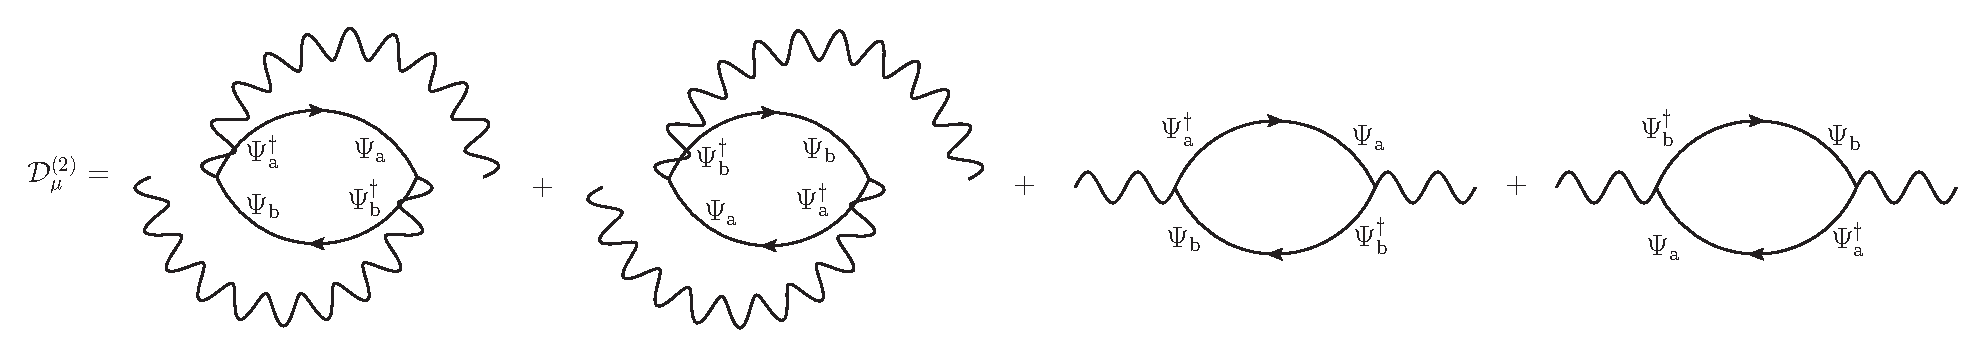
\includegraphics[width=\textwidth]{all_contained_bubble_diagrams.eps}
	\caption{caption}
	\label{fig: all contained bubble diagrams}
\end{figure}
%
On the one hand the acting point of the bosonic lines is changed comparing the first two and last two diagrams.
On the other hand the direction of the electronic lines is interchanged between the first two diagrams and in equal measure for the last two diagrams.
For example, in the first diagram an a-electron is annihiliated and a b-electron is created at $t_{1}$.
Comparing the second diagram, where an a-electron is created and a b-electron is annihilated at $t_{1}$.
All four diagrams are closly connected with each other, because all diagrams can be generated out of one diagram by interchanging the acting point of the bosonic lines or the direction of the fermionic lines.
Therefore all four diagrams yield the same contribution, where it is enough to compute one of them and multiply by four.
%
\begin{align}
	\mathcal{D}_{\mu}^{(2)}(\vb{k}, t-t') &= 
		4i \lambda^{2}
		\int\limits_{-\infty}^{\infty} \dd{t_{1}} \dd{t_{2}}
		\sum\limits_{\vb{P}} \int_{\vb{p}}
		\notag \\ &\times
		\expval{\mathcal{T}_{t} \Phi_{\mu} (\tilde{\vb{k}},t_{2}) \Phi_{\mu}(-\tilde{\vb{k}},t')}_{0}	
		\expval{\mathcal{T}_{t} \Phi_{\mu} (-\tilde{\vb{k}},t_{1}) \Phi_{\mu}(\tilde{\vb{k}},t)}_{0}
		\notag \\ &\times
		\expval{\mathcal{T}_{t} \Psi_{\mt{a}}(\tilde{\vb{p}}-\tilde{\vb{k}},t_{1}) \Psi_{\mt{a}}^{\dag}(\tilde{\vb{p}}-\tilde{\vb{k}},t_{2})}_{0}
		\expval{\mathcal{T}_{t} \Psi_{\mt{b}}(\tilde{\vb{p}},t_{2}) \Psi_{\mt{b}}^{\dag}(\tilde{\vb{p}},t_{1})}_{0}
		\label{eq: spin density wave propagator second order correction}
\end{align}
%
where the momentums $\vb{p}_{1}$ and $\vb{P}_{1}$ are relabeled with $\vb{p}$ and $\vb{P}$, respectivily.
Accordingly we write $\tilde{\vb{p}}$ instead of $\tilde{\vb{p}}_{1}$.
In comparison to the Dyson equation \eqref{eq: Dyson equation} the fermionic bubble is identified with the self energy $\Pi_{\mu}$, where the bubble diagram surely only represented the zeroth order of the self energy.
The self energy in zeroth order is therefore given by
%
\begin{align}
	\Pi_{\mu}^{(0)}(\vb{k}, \omega) = 
		i 
		\sum\limits_{\vb{P}}
		\int\limits_{|p| \leq |p_{\mt{F}}} \frac{\dd[2]{\vb{p}}}{(2\pi)^{2}} 
		\int\limits_{-\infty}^{\infty} \frac{\dd{\epsilon}}{2\pi}\,
		\mathcal{G}_{\mt{a}}^{(0)}(\vb{p}+\frac{\vb{k}}{2}, \epsilon+\frac{\omega}{2})
		\mathcal{G}_{\mt{b}}^{(0)}(\vb{p}-\frac{\vb{k}}{2}, \epsilon-\frac{\omega}{2}).
\end{align}
%
In comparison to equation \eqref{eq: spin density wave propagator second order correction} the self energy is represented in frequency space.
Further the outer momentum and frequency is shifted by the half of itself, so that both arguments of the fermionic propagators are symmetricly, which is depicted in figure \ref{fig: bubble diagram}.
%
\begin{figure}[t]
	\centering
	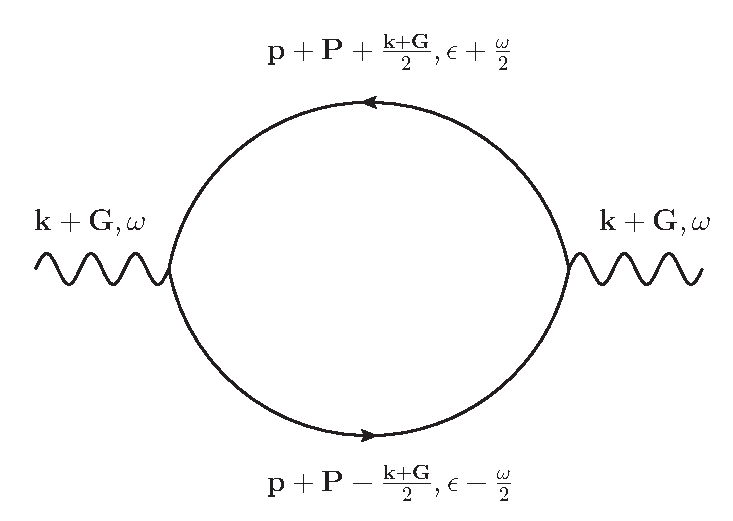
\includegraphics[width=0.5\textwidth]{bubble_diagram.eps}
	\caption{caption}
	\label{fig: bubble diagram}
\end{figure}
%
How we see in equation \eqref{eq: free electron propagator} the free electron propagator contains the dispersion relation $\epsilon_{\alpha}(\vb{p}+\vb{P})$ of the respective electrons.
In our considered spin fermion model only electrons near the Fermi surface interacte with each other interfered by spin density waves, which means that the momentum and energy transfer is small.
Under this condition the dispersion relation can be expanded near the Fermi surface.
%
\begin{align}
	\epsilon_{\mt{a}}(\vb{p} + \vb{P} + \frac{\vb{k} + \vb{G}}{2}) &= 
		\frac{\big(p_{x} + P_{x} + \frac{k_{x} + G_{x}}{2}\big)^{2}}{2m_{1}} 
		+ 
		\frac{\big(p_{y} + P_{y} + \frac{k_{y} + G_{y}}{2}\big)^{2}}{2m_{2}} 
		\notag \\ 
	\Leftrightarrow\ \epsilon_{\mt{a}}(\vb{p} + \vb{P} + \frac{\vb{k} + \vb{G}}{2}) &=
		\frac{(p_{x} + P_{x})^{2}}{2m_{1}} + \frac{1}{2} \frac{p_{x}+P_{x}}{m_{1}}(k_{x}+G_{x}) + \frac{(k_{x}+G_{x})^{2}}{8m_{1}}
		\notag \\ &+
		\frac{(p_{y} + P_{y})^{2}}{2m_{2}} + \frac{1}{2} \frac{p_{y}+P_{y}}{m_{2}}(k_{y}+G_{y}) + \frac{(k_{y}+G_{y})^{2}}{8m_{2}}
		\notag \\
	\Leftrightarrow\ \epsilon_{\mt{a}}(\vb{p} + \vb{P} + \frac{\vb{k} + \vb{G}}{2}) &\approx
		\xi_{\mt{a}} + \frac{1}{2} \vb{v}_{\mt{a,F}}(\vb{k} + \vb{G}) + \mu
\end{align} 
%
where the quadratic term with respect to $\vb{k}$ is neglectable, because the bosonic transfered momentum is assumed as small.
Further the velocity $\vb{v}_{a}$ of the a-electrons is introduced, where the elelctron velocity can be approximated with the Fermi velocity of the corresponding Fermi surface, because only electrons near the Fermi surface are considered.
Besides the dispersion relation $\xi_{\mt{a}}$ of the a-electrons is used, which is given by \dots \todo{link zur dispersion im spin fermion model}.
The same procedure is done for the b-electrons.
Finally the normalized momentum vector $\vb{n} = \frac{\vb{p}+\vb{P}}{|\vb{p}+\vb{P}|}$ is introduced.
The Fermi velocity of the a-electrons is then given by $\vb{v}_{\mt{a,F}} = v_{\mt{a,F}} \vb{n}$ for example.
The scalar product between the normalized momentum vector $\vb{n}$ and the bosonic spin density wave vector $\vb{k} + \vb{G}$ is rewriten as his magnitude multiplied with $\cos(\vartheta)$, where $\vartheta$ is the angle between both.

In the investigated spin fermion model the electrons on different Fermi surfaces only interacte on so called hot spots like we have it introduced in chapter \ref{ch: spin fermion model}.
The energy and the magnitudes of the Fermi velocities are equal on the hot spots.
%
\begin{align}
	\xi := \xi_{\mt{a}} = \xi_{\mt{b}} \qquad v_{\mt{F}} := v_{\mt{a,F}} = v_{\mt{b,F}}
\end{align}
%
Consider that the direction of the velocities haven't been equal, otherwise the angle $\vartheta$ is $0$ or $\pi$ and the imaginary part of $\Pi_{\mu}$ is zero.
Using these assumptions the self energy is given by
%
\begin{align}
	\Pi_{\mu}^{(0)}(\vb{k}, \omega) &= 
		i \nu_{\mt{F}}
		\int\limits_{0}^{\pi} \dd{\vartheta}
		\int\limits_{\xi \leq \xi_{\mt{F}}} \dd{\xi}
		\int\limits_{-\infty}^{\infty} \frac{\dd{\epsilon}}{2\pi}
		\notag \\ &\times
		\frac{1}{\epsilon + \frac{\omega}{2} - \xi - \frac{1}{2} v_{\mt{F}} |\vb{k} + \vb{G}| \cos(\vartheta) + i \eta \sign(\epsilon + \frac{\omega}{2})}
		\notag \\ &\times
		\frac{1}{\epsilon - \frac{\omega}{2} - \xi + \frac{1}{2} v_{\mt{F}} |\vb{k} + \vb{G}| \cos(\vartheta) + i \eta \sign(\epsilon - \frac{\omega}{2})},
	\label{eq: self energy before epsilon integration}
\end{align}
%
where the two dimensional momentum integral is firstly transformed in plane polar coordinates and then the $k$-integral is transformed into an energy integral over the density of states.
Because only electrons near the Fermi surface are considered the density of states can be approximated with the constant one $\nu_{\mt{F}} := \nu(\xi_{\mt{F}})$ at the Fermi surface.
The energy integral is certainly limited by the Fermi energy $\xi_{\mt{F}}$.

The further investigation is been starting with the computation of the frequency integral.
Therefore the integral over $\epsilon$ is transformed into a complex contour integral, where the contour $\Gamma$ is chosen in two different ways.
In both case the contour starts along the real axis.
According to the singularities of the integrand the countour is closed in the upper or lower half plane via a semicircle with radius infinity.
In both cases the contribution of the semicircle is zero because the integrand is proportional to $\flatfrac{1}{\epsilon}$.
The non-contributing of the semicircle ensures the equality between the integral along the real axis and the complex contour integral.
The investigated integrand occupies two singularities at
%
\begin{align}
	\epsilon_{1} := \xi - \frac{1}{2}\big(\omega - v_{\mt{F}} |\vb{k} + \vb{G}| \cos(\vartheta)\big) 
	\qq{and}
	\epsilon_{2} := \xi + \frac{1}{2}\big(\omega - v_{\mt{F}} |\vb{k} + \vb{G}| \cos(\vartheta)\big),
\end{align}
%
where both singularities are of first order which allows using Cauchy's integral formula.
According to the signum function in both denominators the poles are located in the upper or lower plane.
So in total there are four different possible constitutions.
On the one hand both singularities can be located in the lower or upper complex plane, which yield in both cases zero.
On the other hand one pole can be in the upper plane and the other one can be in the lower plane, or vice versa.
Equally both constitutions yields the same contribution.
%
\paragraph{1. case:} $\sign(\epsilon + \frac{\omega}{2}) = \sign(\epsilon - \frac{\omega}{2})$\\
%
Both singularities are located in the upper or in the lower complex half plane.
The contour is therefore closed in the upper or lower plane, respectivily, so that both poles are enclosed.
In the first case the winding number is $1$, because the pole is enclosed counterclockwise.
Accordingly the winding number is $-1$ in the second case.
%
\begin{align}
	&\mt{I}_{\omega}^{\mt{e}} := i \oint_{\Gamma} \frac{\dd{\omega}}{2\pi i}\, \frac{1}{\omega - \omega_{1} \mp i\eta} \cdot \frac{1}{\omega - \omega_{2} \mp i\eta}
	\notag \\
	\Leftrightarrow\ &\mt{I}_{\omega}^{\mt{e}} = \pm i \bigg[ \frac{1}{\omega_{2} - \omega_{1}} + \frac{1}{\omega_{1} - \omega_{2}}\bigg] = 0,
\end{align}
%
where the index "e" stands for even and should mean that both poles are located at the same half planes.
%
\paragraph{2. case:} $\sign(\epsilon + \frac{\omega}{2}) \neq \sign(\epsilon - \frac{\omega}{2})$\\
%
The singularities are located in different complex half planes, one in the upper and accordingly the other in the lower half plane.
In both cases it's arbitrary how the contour is closed.
It's only important that one of the two poles is located inside the contour.
In the following computation the contour is closed in the upper half plane, so the winding number is always $1$.
%
\begin{align}
	&\mt{I}_{\omega}^{\mt{o}} := i \oint_{\Gamma} \frac{\dd{\omega}}{2\pi i}\, \frac{1}{\omega - \omega_{1} \mp i\eta} \cdot \frac{1}{\omega - \omega_{2} \pm i\eta}
	\notag \\
	\Leftrightarrow\ &\mt{I}_{\omega}^{\mt{o}} = \frac{\pm i}{\omega_{2} - \omega_{1} \pm i\eta}
\end{align}
%
where the index "o" stands accordingly for odd and should mean that both poles are located in different half planes.

Inserting both singularities $\omega_{1}$ and $\omega_{2}$ causes that the integrand is independent with respect to the energy $\xi$.
The frequency depending signum functions in \eqref{eq: self energy before epsilon integration} is aquivalent to the signum functions $\sign(\xi \pm \frac{1}{2} v_{\mt{F}} |\vb{k} + \vb{G}| \cos(\vartheta))$ in energy representation.
The energy $\xi$ is neglectable because the integrand is independent of $\xi$.
Further the constant factors are also neglectable because them are always positive. 
The case of sign in the integand depends therefore only on the sign of $|\vb{k} + \vb{G}| \cos(\vartheta)$.
Finally the integrals limits has to be set to $\pm \frac{1}{2} v_{\mt{F}} |\vb{k} + \vb{G}| \cos(\vartheta)$.
This follows directly from the location of the poles.
For example if $\omega_{1}$ is in the lower and $\omega_{2}$ is in the upper half plane than $\epsilon + \frac{\omega}{2} > 0$ and $\epsilon - \frac{\omega}{2} < 0$, respectivily.
Transforming both into energy representation the corresponding expressions are $\xi - \frac{1}{2} v_{\mt{F}} |\vb{k} + \vb{G}| \cos(\vartheta) < 0$ and $\xi + \frac{1}{2} v_{\mt{F}} |\vb{k} + \vb{G}| \cos(\vartheta) > 0$, which yields directly the definition interval of $\xi$.
Therefore we obtained 
%
\begin{align}
	\Pi_{\mu}^{(0)}(\vb{k}, \omega) &= 
		i \nu_{\mt{F}}
		\int\limits_{0}^{\pi} \dd{\vartheta} 
		\int\limits_{-\xi_{0}}^{\xi_{0}} \dd{\xi}
		\frac{i \sign(|\vb{k} + \vb{G}| \cos(\vartheta))}{\omega - v_{\mt{F}} |\vb{k} + \vb{G}| \cos(\vartheta) + i\eta \sign(|\vb{k} + \vb{G}| \cos(\vartheta))}
\end{align}
%
for the self energy, where the abbreviation $\xi_{0} = \flatfrac{v_{\mt{F}}|\vb{k}+\vb{G}|\cos(\vartheta)}{2}$ is introduced.
The integration over $\xi$ yields the factor $v_{\mt{F}}|\vb{k}+\vb{G}|\cos(\vartheta)$.
Subsequently the signum function is reexpressed in frequency representation which corresponds to $\sign(\omega)$.

Like it is shown above the damping of the spin density wave occurs of the imaginary part of the self energy, which is the reason why we take the imaginary part of the above expression in the further computation.
%Formally the real part is absorbed into the mass term $r_{0}$.
The imaginary part of the serlf energy is given by
%
\begin{align}
	\Im{\Pi_{\mu}^{(0)}(\vb{k}, \omega)} &= 
		\nu_{\mt{F}} \pi
		\int\limits_{0}^{\pi} \dd{\vartheta}
		v_{\mt{F}} |\vb{k}+\vb{G}| \cos(\vartheta) \delta(\omega - v_{\mt{F}} |\vb{k} + \vb{G}| \cos(\vartheta)),
	\label{eq: imaginary part of self energy before theta integration}
\end{align}
%
where the formula $\frac{1}{x \pm i\eta} = \PV{\frac{1}{x}} \mp i \pi \delta(x)$ is used.
To perform the last remaining intgeral over $\vartheta$ the $\delta$-distribution has to be rewriten.
The argument is a $\vartheta$ depending function with in general infinite zeros.
But in the integrating area, between $0$ and $\pi$, the cosine only have one zero.
The formula
%
\begin{align}
	\delta(g(x)) = \sum\limits_{i=1} \frac{\delta(x-x_{0,i})}{|g'(x_{0,i})|}
\end{align}
%
states how a $\delta$-distribution with a functional argument can be writen as a sum over $\delta$-distributions with zeros of $g(x)$ as arguments.
The prime denotes the derivative with respect to $x$ which has to be evaluated at the corresponding zero $x_{0,i}$.
The argument of the $\delta$-distribution in \eqref{eq: imaginary part of self energy before theta integration} has a single zero at $\vartheta_{0} = \cos[-1](\flatfrac{\omega}{(v_{\mt{F}} |\vb{k} + \vb{G}|)})$.
Thereby the $\delta$-distribution is rewriten as
%
\begin{align}
	&\delta(\omega - v_{\mt{F}} |\vb{k} + \vb{G}| \cos(\vartheta)) = \Big(v_{\mt{F}} |\vb{k} + \vb{G}| \cdot |\sin(\vartheta_{0})|\Big)^{-1} \delta(\vartheta - \vartheta_{0})
	\notag \\
	\Rightarrow\ &\delta(\omega - v_{\mt{F}} |\vb{k} + \vb{G}| \cos(\vartheta)) \approx \Big(v_{\mt{F}} |\vb{k} + \vb{G}|\Big)^{-1} \delta(\vartheta - \vartheta_{0})
\end{align}
%
where in the second line the limit of small frequancies $\omega$ is performed.
This is valid because of our investigated low energy theory.
In other words the interaction is assumed as small and thereby the frequency and momentum transfer is small too.
Now the integration over $\vartheta$ can be performed easily.
The imaginary part of the self energy is given by
%
\begin{align}
	\Im{\Pi_{\mu}^{(0)}(\vb{k}, \omega)} &= \frac{\nu_{\mt{F}} \pi}{v_{\mt{F}} |\vb{k} + \vb{G}|} \cdot \omega = \gamma \omega		 
\end{align}
%
where in the last step the damping constant $\gamma$ is introduced.
In equation \eqref{eq: Dyson equation} we see that the full propagator is given by the free propagator and the self energy.
In general the self energy is a complex quantity why they is splitted into real and imaginary part.
With the free propagator in equation \eqref{eq: free spin density wave propagator} the damped spin fermion propagator is given by
%
\begin{align}
	\mathcal{D}_{\mu}(\vb{k}, \omega) = \sum\limits_{\vb{G}} \frac{1}{(\vb{k}+\vb{G})^{2} + r - \xi^{-2} - i \gamma \omega}
	\label{eq: damped spin density propagator with real omega}
\end{align}
%
where the abbreviation $r = r_{0} - \Re{\Pi_{\mu}(\vb{k}, \omega)}$ is used.
Remember that $\xi$ represents the correlation length in this formula instead of the energy like it's used in the previous computation.
At the quantum critical point the even introduced quantity $r$ is zero.
The real part of self energy is canceled with $r_{0}$.
Further the investigated model is a low energy theory, why the correlation length $\xi$, which is proportional to $\omega^{2}$ is neglectable.
%
%
\section{Transformation of the propagator on the imaginary axis}
\label{sec: transformation of the propagator on the imaginary axis}
%
%
The spin density wave propagator obtained in the previous section is a complex function of the real quantity $\omega$.
In the following the quantity $\omega$ should be transformed into an imaginary quantity $i\omega_{n}$, which we know as Matsubara frequancies.
In this representation the computations in chapter \ref{ch: calculation} are much more convienent.
The aim is now to find the real and imaginary part of the propagator with respect to the imaginary quantity $i\omega_{n}$.
The Kramers-Kronig relations yield a relationship between the real part of a function and the imaginary part of the same function, or vice versa, where the argument of both parts is rotated by an arbitrary angle.
In section \ref{subsec: Kramer-Kronig-relation} these relations are established, see \eqref{eq: Kramer-Kronig relation} for the explicite form.
The propagator in \eqref{eq: damped spin density propagator with real omega} can be easily seperated into real and imaginary part
%
\begin{align}
	\mathcal{D}_{\mu}(\vb{k}, \omega) = \sum\limits_{\vb{G}} \bigg[\frac{(\vb{k}+\vb{G})^{2}}{(\vb{k}+\vb{G})^{4} + (\gamma\omega)^{2}} + i \frac{\gamma \omega}{(\vb{k}+\vb{G})^{4} + (\gamma\omega)^{2}}\bigg],
\end{align}
%
where $r = \xi = 0$ is set.
It is trivially seen that the real part is a symmetric function and the imaginary part is an antiysmmetric funtion with respect to $\omega$.
Similiar to \eqref{eq: damped spin density propagator with real omega} the propagator $\mathcal{D}_{\mu}(\vb{k}, i\omega_{n})$ can be seperated into a real and imaginary part.
The imaginary part is zero, because the integrand in \eqref{eq: Kramer-Kronig relation} is an antisymmetric function with respect to $\omega$.
So the propagator with respect to Matsubara frequencies is given by
%
\begin{align}
	\mathcal{D}_{\mu}(\vb{k}, i\omega_{n}) = \frac{1}{\pi} \PV{\int\limits_{-\infty}^{\infty} \dd{\omega} \frac{\Im{\mathcal{D}_{\mu}(\vb{k}, \omega)}}{\omega - i\omega_{n}}}
\end{align}
%
The integral is splitted into two parts and in the first term we substitute with $\omega = -\omega$ and the antismmetry of $\Im{\mathcal{D}_{\mu}(\vb{k}, \omega)}$ is utilizied.
%
\begin{align}
	%&\mathcal{D}_{\mu}(\vb{k}, i\omega_{n}) = \frac{1}{\pi} \Bigg[
	%	\int\limits_{-\infty}^{0} \dd{\omega} \frac{\Im{\mathcal{D}_{\mu}(\vb{k}, \omega)}}{\omega - i\omega_{n}}
	%	+
	%	\int\limits_{0}^{\infty} \dd{\omega} \frac{\Im{\mathcal{D}_{\mu}(\vb{k}, \omega)}}{\omega - i\omega_{n}}
	%\Bigg]
	%\notag \\
	%\Leftrightarrow\ 
	&\mathcal{D}_{\mu}(\vb{k}, i\omega_{n}) = \frac{1}{\pi} \int\limits_{0}^{\infty} \dd{\omega} \Im{\mathcal{D}_{\mu}(\vb{k}, \omega)} \Bigg[
		\frac{1}{\omega + i\omega_{n}}
		+
		\frac{1}{\omega - i\omega_{n}}
	\Bigg]
	\notag \\
	\Leftrightarrow\ &\mathcal{D}_{\mu}(\vb{k}, i\omega_{n}) = 
		\frac{2}{\pi} \sum\limits_{\vb{G}} \int\limits_{0}^{\infty} \dd{\omega} 
		\frac{\gamma \omega}{(\vb{k}+\vb{G})^{4} + (\gamma\omega)^{2}} \cdot
		\frac{\omega}{\omega^{2} + \omega_{n}^{2}}
	\notag \\
	\Leftrightarrow\ &\mathcal{D}_{\mu}(\vb{k}, i\omega_{n}) = 
		\sum\limits_{\vb{G}} \frac{1}{(\vb{k}+\vb{G})^{2} + \gamma|\omega_{n}|}
	\label{eq: damped propagator Matsubara representation}
\end{align}
%
In the last step the integral formula
%
\begin{align}
	\int\limits_{0}^{\infty} \dd{x} \frac{x}{a^{2} + x^{2}} \cdot \frac{x}{y^{2} + x^{2}} = \frac{\pi}{2} \frac{1}{a + |y|}
\end{align}
%
is used, which can be shown by transforming into a complex contour integral.


















